\chapter{Dynamic System Modeling}
\label{ch:sysModeling}

The goal of this section is to derive a preliminary state-space model for the MARGE in the form
\begin{equation}
\label{eq:modelingGoal}
	\begin{aligned}
    		s \{x\} &= [A] \{x\} + [B]\{u\} \\
	    \{y\} &= [C] \{x\} + [D] \{u\}
	\end{aligned}
\end{equation}
based on first principles.

%%%%%%%%%%%%%%%%%%%%%%%%%%%%%%%%%%%%%%%%%%%%%%%%%%%%%%%%%%%%%%%%%%%%%%%%
\section{Plant Dynamics} %%%%%%%%%%%%%%%%%%%%%%%%%%%%%%%%%%%%%%%%%%%%%%%
%%%%%%%%%%%%%%%%%%%%%%%%%%%%%%%%%%%%%%%%%%%%%%%%%%%%%%%%%%%%%%%%%%%%%%%%

This section will derive the plant dynamics for MARGE in the form
\begin{align}
	\label{eq:ssPlant}
	s \{x\} = [A_p]\{x_p\}+[B_p]\{u_p\}
\end{align}

\subsection{Structural Dynamics} %%%%%%%%%%%%%%%%%%%%%%%%%%%%%%%%%%%

MARGE's structure is modeled as a linear, second-order system with damping and external forcing. The equations of motion for such a system are
\begin{align}
    s^2 [M] \{q(s)\} + s [C] \{q(s)\} + [K] \{q(s)\} &= \{f(s)\}
\end{align}
where $\{q\}$ is the structural dynamic state expressed in generalized modal coordinates, $\{f(s)\}$ is the generalized external forcing, and $[M]$, $[C]$, and $[K]$ are generalized mass, damping, and stiffness matrices respectively. Note that the modal coordinates include both elastic motions (of the structure) denoted by the subscript $s$ and rigid-body motions (of the structure and the control surfaces) denoted by the subscript $c$:
\begin{align}
    \{q\} = \begin{Bmatrix} q_{s} \\ q_{c} \end{Bmatrix}
\end{align}
% The mass matrix, and stiffness matrix, and the mode shapes corresponding to $\{q\}$ are obtained from the NASTRAN model.

% The forcing for the aeroservoelastic wing can be decomposed into the aerodynamic forcing due to the state, the aerodynamic forcing due to gusts, and the forcing from actuator hinge moments:
% \begin{align}
%     s^2 [M] \{q(s)\} + s [C] \{q(s)\} + [K] \{q(s)\} &= q_D [A(s)] \{q(s)\} + q_D [A_G(s)] \frac{w_G}{U} + \begin{Bmatrix} \{0\} \\ \{H_c\} \end{Bmatrix}
% where $[A]$ is the aerodynamic influence matrix for the state, $[A_G]$ is the aerodynamic influence matrix for gusts, and ${H_c}$ is the hinge moment's influence.
The forcing for the aeroservoelastic wing can be decomposed into the aerodynamic forcing due to the state and the forcing from actuator hinge moments:
\begin{align}
    s^2 [M] \{q(s)\} + s [C] \{q(s)\} + [K] \{q(s)\} &= q_D [A(s)] \{q(s)\} + \begin{Bmatrix} \{0\} \\ \{H_c\} \end{Bmatrix}
\end{align}
where $[A(s)]$ is the aerodynamic influence matrix for the state and $\{H_c\}$ are the hinge moments from the actuators.

The whole system can be further decomposed into structural and control components:
\begin{multline}
    \left( s^2 \begin{bmatrix}
        [M_{ss}] & [M_{sc}] \\
        [M_{cs}] & [M_{cc}]
    \end{bmatrix} + s \begin{bmatrix}
        [C_{ss}] & [C_{sc}] \\
        [C_{cs}] & [C_{cc}]
    \end{bmatrix} + \begin{bmatrix}
        [K_{ss}] & [K_{sc}] \\
        [K_{cs}] & [K_{cc}]
    \end{bmatrix} \right) \begin{Bmatrix}
        \{q_s(s)\} \\
        \{q_c(s)\}
    \end{Bmatrix} \\ = q_D \begin{bmatrix}
        [A_{ss}(s)] & [A_{sc}(s)] \\
        [A_{cs}(s)] & [A_{cc}(s)]
    \end{bmatrix} \begin{Bmatrix}
        \{q_s(s)\} \\
        \{q_c(s)\}
    \end{Bmatrix}
    % + q_D \begin{bmatrix}
    %     [A_{G,ss}(s)] & [A_{G,sc}(s)] \\
    %     [A_{G,cs}(s)] & [A_{G,cc}(s)]
    % \end{bmatrix} \frac{w_G}{U}
    + \begin{Bmatrix}
        \{0\} \\
        \{H_c\}
    \end{Bmatrix}
\end{multline}
The control modes are those corresponding to rigid-body motions of control surfaces. The structural modes are all other modes, including flexible-body modes and rigid-body pitching of the entire model.

It is assumed that the dynamics of the control modes are completely determined by the control inputs and the inputs are not directly affected by the control modes, i.e. the actuators are irreversible controls. Then, interest is only in the dynamics of the structural modes:
\begin{multline}
    \left( s^2 \begin{bmatrix}
        [M_{ss}] & [M_{sc}]
    \end{bmatrix} + s \begin{bmatrix}
        [C_{ss}] & [C_{sc}]
    \end{bmatrix} + \begin{bmatrix}
        [K_{ss}] & [K_{sc}]
    \end{bmatrix} \right) \begin{Bmatrix}
        \{q_s(s)\} \\
        \{q_c(s)\}
    \end{Bmatrix} \\ = q_D \begin{bmatrix}
        [A_{ss}(s)] & [A_{sc}(s)]
    \end{bmatrix} \begin{Bmatrix}
        \{q_s(s)\} \\
        \{q_c(s)\}
    \end{Bmatrix}
    % + q_D \begin{bmatrix}
    %     [A_{G,ss}(s)] & [A_{G,sc}(s)]
    % \end{bmatrix} \frac{w_G}{U}
\end{multline}

Note that since the control modes are rigid-body modes, they have no stiffness and the equations of motion further simplify to
\begin{multline}
	\label{eq:EOM}
    \left( s^2 \begin{bmatrix}
        [M_{ss}] & [M_{sc}]
    \end{bmatrix} + s \begin{bmatrix}
        [C_{ss}] & [C_{sc}]
    \end{bmatrix} + \begin{bmatrix}
        [K_{ss}] & [0]
    \end{bmatrix} \right) \begin{Bmatrix}
        \{q_s(s)\} \\
        \{q_c(s)\}
    \end{Bmatrix} \\ = q_D \begin{bmatrix}
        [A_{ss}(s)] & [A_{sc}(s)]
    \end{bmatrix} \begin{Bmatrix}
        \{q_s(s)\} \\
        \{q_c(s)\}
    \end{Bmatrix}
    % + q_D \begin{bmatrix}
    %     [A_{G,ss}(s)] & [A_{G,sc}(s)]
    % \end{bmatrix} \frac{w_G}{U}
\end{multline}

\subsection{The Roger Approximation} %%%%%%%%%%%%%%%%%%%%%%%%%%%%%%%

% The aerodynamic influence matrices $[A]$ and $[A_G]$ are nonlinear functions of frequency. In order to obtain a linear state-space system, these must be approximated as analytic functions of $s$.
The aerodynamic influence matrix $[A]$ is a function of the Laplace variable $s$. For a thin airfoil oscillating in a potential flow, Theodorsen's analytical solution applies \cite{Theodorsen1949}. In the more general case of an aircraft's wing in three dimensions, a numerical solver using doublet-lattice theory can compute $[A]$. This solution is nonlinear and unable to be represented in a linear system. In order to obtain the linear state-space system, $[A]$ must be approximated as an analytic function of $s$.

The Roger approximation \cite{Roger1977} is a method of generating a rational function approximation of the aerodynamic influence matrix in the form
\begin{align}
	\label{eq:RogerApprox}
    [A(s)] \approx [P_0] + s [P_1] + s^2 [P_2] + \sum_{n=1}^{N_\text{lag}} \frac{s}{s+\beta_n} [P_{n+2}]
\end{align}
where $[P]$ are the unknown real-valued matrices that are fit to tabulated known $[A(s)]$ matrices (obtained from an unsteady aerodynamic solver such as that found in NASTRAN). Aside from the zeroth, first, and second order terms, there are $N_\text{lag}$ additional ``lag term'' approximating functions which are defined by their respective constants $\beta$. These constants $\beta$ are chosen by the user.

Begin with an approximation only along the frequency domain:
\begin{align}
    [A(jk)] &\approx [\bar{P}_0] + jk [\bar{P}_1] + (jk)^2 [\bar{P}_2] + \sum_{n=1}^{N_\text{lag}} \frac{jk}{jk+\bar{\beta}_n} [\bar{P}_{n+2}]
\end{align}
where $k$ is the reduced frequency
\begin{align}
	k = \frac{\omega \cdot b}{U}
\end{align}
Given the tabulated set of aerodynamic influence matrices $[A]$ computed across $N$ reduced frequencies, each entry $p$ of the matrices $[\bar{P}]$ in the above approximation can be fit to the corresponding entries $a$ of the aerodynamic influence matrices $[A]$. The steady-state component of the approximation $[\bar{P}_0]$ is fixed to be equal to the steady-state aerodynamic influence matrix (with zero reduced frequency):
\begin{align}
    [\bar{P}_0] &= [A(k=0)]
\end{align}
The remaining $[\bar{P}]$ matrices are determined using a linear regression:
\begin{align}
	\label{eq:RogerRegression}
    \begin{bmatrix}
        0 & -k_1^2 & \frac{k_1^2}{k_1^2 + \bar{\beta}_1^2} & \dots & \frac{k_1^2}{k_1^2 + \bar{\beta}_{N_\text{lag}}^2} \\
	    k_1 & 0 & \frac{k_1 \bar{\beta}_1}{k_1^2 + \bar{\beta}_1^2} & \dots & \frac{k_1 \bar{\beta}_1}{k_1^2 + \bar{\beta}_{N_\text{lag}}^2} \\
	    \vdots & \vdots & \vdots & & \vdots \\
        0 & -k_N^2 & \frac{k_N^2}{k_N^2 + \bar{\beta}_1^2} & \dots & \frac{k_N^2}{k_N^2 + \bar{\beta}_{N_\text{lag}}^2} \\
	    k_N & 0 & \frac{k_N \bar{\beta}_1}{k_N^2 + \bar{\beta}_1^2} & \dots & \frac{k_N \bar{\beta}_1}{N^2 + \bar{\beta}_{N_\text{lag}}^2}	    
    \end{bmatrix}
    \begin{Bmatrix} \bar{p}_1 \\ \vdots \\ \bar{p}_{N_\text{lag}+2} \end{Bmatrix}
    &=
    \begin{Bmatrix}
	    \Re(a(jk_1)) - a(0) \\
	    \Im(a(jk_1)) \\
	    \vdots \\
	    \Re(a(jk_N)) - a(0) \\
	    \Im(a(jk_N))	    
    \end{Bmatrix}
\end{align}
The linear regression in Eq. \ref{eq:RogerRegression} can then be solved using the method of least-squares to obtain the fitted $[\bar{P}]$ matrices.
% With these matrices, Eq. \ref{eq:RogerApprox} is a known rational approximation for the aerodnyamic influence matrices across the tabulated natural frequencies. Replacing the aerodynamic influence matrices in Eq. \ref{eq:EOM} yields a fully linear model for structural dynamics of MARGE.

Replacing the reduced frequency with the equivalent angular frequency yields
\begin{align}
	[A(j\omega)] \approx [P_0] + j\omega [P_1] - \omega^2 [P_2] + \sum_{n=1}^{N_\text{lag}} \frac{j\omega}{j\omega+\beta_n} [P_{n+2}]
\end{align}
where
\begin{equation}
\begin{aligned}
	[P_0] &= [\bar{P}_0] \\
	[P_1] &= [\bar{P}_1] \frac{b}{U} \\
	[P_2] &= [\bar{P}_2] \left(\frac{b}{U}\right)^2 \\
	[P_3] &= [\bar{P}_3] \\
	&\vdots \\
	[P_{N_\text{lag}+2}] &= 	[\bar{P}_{N_\text{lag}+2}] \\
	\beta_1 &= \bar{\beta}_1 \frac{U}{b} \\
	&\vdots \\
	\beta_{N_\text{lag}} &= \bar{\beta}_{N_\text{lag}} \frac{U}{b}
\end{aligned}
\end{equation}
This is then extended from the imaginary axis to the full Laplace domain through analytic continuation, leading to the final form of the Roger approximation for aerodynamic influence matrices:
\begin{align}
	[A(s)] \approx [P_0] + s [P_1] + s^2 [P_2] + \sum_{n=1}^{N_\text{lag}} \frac{s}{s+\beta_n} [P_{n+2}]
\end{align}

It should be noted that the Roger approximation is only valid over the tabulated reduced frequency range. Thus, any result from the model is only valid if the airspeed that the model ia analyzed at is sufficiently above
\begin{align}
	U_\text{min} &= \frac{\omega_\text{max} \cdot b}{k_\text{max}}
\end{align}
where $\omega_\text{max}$ is the maximum frequency of interest in the analysis. Thus, modeling which utilizes the Roger Approximation cannot be used for purely structural dynamic analysis (where $U=0$).

\subsection{Coupled Aeroelastic Dynamics} %%%%%%%%%%%%%%%%%%%%%%%%%%

This section describes how the structural dynamic equations of motion can be reduced to the form in Eq. \ref{eq:ssPlant}.

Replacing the aerodynamic influence matrices in Eq. \ref{eq:EOM} with the equivalent Roger approximation and collecting like terms yields
\begin{multline}
	\label{eq:EOMwRoger}
	\left( s^2 [M_{ss}] + s [C_{ss}] + [K_{ss}]
	- q_D \left( [P_{ss,0}] + s[P_{ss,1}] + s^2 [P_{,2}] + \sum_{n=1}^{N_\text{lag}} \frac{s}{s+\beta_n} [P_{ss,n+2}] \right) \right) \{ q_s(s)\} \\
	=
	- \left( s^2 [M_{sc}] + s [C_{sc}] - q_D \left( [P_{sc,0}] + s [P_{sc,1}] + s^2 [P_{sc,2}] + \sum_{n=1}^{N_\text{lag}} \frac{s}{s+\beta_n} [P_{sc,n+2}] \right) \right) \{q_c(s)\}
\end{multline}

Define the following coupled aeroelastic mass, damping, and stiffness matrices:
\begin{equation}
\begin{aligned}
	\left[\bar{\bar{M}}\right] &= [M] - q_D [P_2] \\
	\left[\bar{\bar{C}}\right] &= [C] - q_D [P_1] \\
	\left[\bar{\bar{K}}\right] &= [K] - q_D [P_0]
\end{aligned}
\end{equation}
Equation \ref{eq:EOMwRoger} then simplifies to
\begin{multline}
	\left( s^2 \left[\bar{\bar{M}}_{ss}\right] + s \left[\bar{\bar{C}}_{ss}\right] + \left[\bar{\bar{K}}_{ss}\right] \right) \{ q_s(s)\}
	- q_D \left(\sum_{n=1}^{N_\text{lag}} \frac{s}{s+\beta_n} [P_{ss,n+2}] \right) \{ q_s(s)\} \\
	=
	- \left( s^2 \left[\bar{\bar{M}}_{sc}\right] + s \left[\bar{\bar{C}}_{sc}\right] + \left[\bar{\bar{K}}_{sc}\right] \right) \{q_c(s)\} + q_D \left(\sum_{n=1}^{N_\text{lag}} \frac{s}{s+\beta_n} [P_{sc,n+2}] \right) \{q_c(s)\}
\end{multline}
Rearranging the lag terms,
\begin{multline}
	\label{eq:EOMcoupled}
	\left( s^2 \left[\bar{\bar{M}}_{ss}\right] + s \left[\bar{\bar{C}}_{ss}\right] + \left[\bar{\bar{K}}_{ss}\right] \right) \{ q_s(s)\}
	\\
	- q_D \begin{bmatrix}
		\sum_{n=1}^{N_\text{lag}} \frac{s}{s+\beta_n} [P_{ss,n+2}] &
		\sum_{n=1}^{N_\text{lag}} \frac{s}{s+\beta_n} [P_{sc,n+2}] &
	\end{bmatrix} \begin{Bmatrix} q_s(s) \\ q_c(s) \end{Bmatrix}
	\\
	= - \left( s^2 \left[\bar{\bar{M}}_{sc}\right] + s \left[\bar{\bar{C}}_{sc}\right] + \left[ \bar{\bar{K}}_{sc} \right] \right) \begin{Bmatrix} q_c(s) \end{Bmatrix}
\end{multline}

Define the following aerodynamic ``lag states'' as
\begin{equation}
\begin{aligned}
	\{r_1\} &= \begin{bmatrix} [P_{ss,3}] & [P_{sc,3}] \end{bmatrix} \frac{s}{s+\beta_1} \\
	&\vdots \\
	\{r_{N_\text{lag}}\} &= \begin{bmatrix} [P_{ss,N_\text{lag}+2}] & [P_{sc,N_\text{lag}+2}] \end{bmatrix} \frac{s}{s+\beta_{N_\text{lag}}}
\end{aligned}
\end{equation}
Rearranging this yields an expression for the first derivative of the lag states:
\begin{equation}
\begin{aligned}
	s \{r_1\} &= s [P_{ss,3}] \{q_s(s)\} + s [P_{sc,3}] \{q_c(s)\} - \beta_1 \{r_1\} \\
	&\vdots \\
	s \{r_{N_\text{lag}}\} &= s [P_{ss,N_\text{lag}+2}] \{q_s\} + s [P_{sc,N_\text{lag}+2}] \{q_c\} - \beta_{N_\text{lag}} \{r_{N_\text{lag}}\}
\end{aligned}
\end{equation}
Combining these lag state dynamic equations into a single matrix equation yields
\begin{align}
	\label{eq:lagDynamics}
	s\{r\} &= s [B_{rs}] \{q_s\} + s [B_{rc}] \{q_c\} + [A_r] \{r\}
\end{align}
where $\{r\}$, $[B_{rs}]$, $[B_{rc}]$, and $[A_r]$ are defined as
\begin{equation}
\begin{aligned}
	\{r\} &= \begin{Bmatrix} \{r_1\} \\ \vdots \\ \{r_{N_\text{lag}}\} \end{Bmatrix} \\
	[B_{rs}] &= \begin{bmatrix} [P_{ss,3}] \\ \vdots \\ [P_{ss,N_\text{lag}+2}] \end{bmatrix} \\
	[B_{rc}] &= \begin{bmatrix} [P_{sc,3}] \\ \vdots \\ [P_{sc,N_\text{lag}+2}] \end{bmatrix}	\\
	[A_r] &= \begin{bmatrix}
	-\beta_1 [I] & & \\
	& \ddots & \\
	& & -\beta_{N_\text{lag}} [I]
	\end{bmatrix}
\end{aligned}
\end{equation}

With the lag states defined, Eq.\ref{eq:EOMcoupled} can now be rewritten as
\begin{multline}
	\label{eq:EOMcoupled2}
	\left( s^2 \left[\bar{\bar{M}}_{ss}\right] + s \left[\bar{\bar{C}}_{ss}\right] + \left[\bar{\bar{K}}_{ss}\right] \right) \{ q_s(s)\}
	- q_D \sum_{n=1}^{N_\text{lag}} \{r_n\}
	\\
	= - \left( s^2 \left[\bar{\bar{M}}_{sc}\right] + s \left[\bar{\bar{C}}_{sc}\right] + \left[\bar{\bar{K}}_{sc}\right] \right) \begin{Bmatrix} q_c(s) \end{Bmatrix}
\end{multline}
The sum of lag states can be simplifed introducing the matrix $[I_r]$ such that
\begin{align}
	\{r_1\} + \dots + \{r_{N_\text{lag}}\}
	&= \begin{bmatrix} [I] & \dots & [I] \end{bmatrix} \begin{Bmatrix} \{r_1\} \\ \vdots \\ \{r_{N_\text{lag}}\} \end{Bmatrix} = [I_r] \{r\}
\end{align}
This further compacts Eq. \ref{eq:EOMcoupled2}, which becomes
\begin{multline}
	\label{eq:EOMcoupled3}
	\left( s^2 \left[\bar{\bar{M}}_{ss}\right] + s \left[\bar{\bar{C}}_{ss}\right] + \left[\bar{\bar{K}}_{ss}\right] \right) \{ q_s(s)\}
	- q_D [I_r] \{r\}
	\\
	= - \left( s^2 \left[\bar{\bar{M}}_{sc}\right] + s \left[\bar{\bar{C}}_{sc}\right] + \left[\bar{\bar{K}}_{sc}\right] \right) \begin{Bmatrix} q_c(s) \end{Bmatrix}
\end{multline}

Define new structural dynamic state vectors as
\begin{align}
	\{x_1\} &= \{q\} \\
	\{x_2\} &= s \{q\}
\end{align}
Using these, Eq. \ref{eq:EOMcoupled3} can be rewritten as a first-order linear ODE for $\{x_2\}$:
\begin{multline}
	s \{x_2\} = - \left[\bar{\bar{M}}_{ss}\right]^{-1} \left[\bar{\bar{C}}_{ss}\right] \{x_2\}
	- \left[\bar{\bar{M}}_{ss}\right]^{-1} \left[\bar{\bar{K}}_{ss}\right] \{x_1\}
	+ q_D \left[\bar{\bar{M}}_{ss}\right]^{-1} [I_r] \{r\}
	\\
	- \left[\bar{\bar{M}}_{ss}\right]^{-1} \left( s^2 \left[\bar{\bar{M}}_{sc}\right] + s \left[\bar{\bar{C}}_{sc}\right] + \left[\bar{\bar{K}}_{sc}\right] \right) \begin{Bmatrix} q_c(s) \end{Bmatrix}
\end{multline}
Rearranging,
\begin{multline}
	\label{eq:EOMcoupled4}
	s\{x_2\} = - \left[\bar{\bar{M}}_{ss}\right]^{-1} \left[\bar{\bar{C}}_{ss}\right] \{x_2\}
	- \left[\bar{\bar{M}}_{ss}\right]^{-1} \left[\bar{\bar{K}}_{ss}\right] \{x_1\}
	\\
	+ q_D \left[\bar{\bar{M}}_{ss}\right]^{-1} [I_r] \{r\}
	- \left[\bar{\bar{M}}_{ss}\right]^{-1}
	\begin{bmatrix}
		\left[\bar{\bar{K}}_{sc}\right] & \left[\bar{\bar{C}}_{sc}\right] & \left[\bar{\bar{M}}_{sc}\right]
	\end{bmatrix}
	\begin{Bmatrix} \{q_c(s)\} \\ s \{q_c(s)\} \\ s^2 \{q_c(s)\} \end{Bmatrix}
\end{multline}

Define the following simplifying matrices:
\begin{align}
	[T_{21}] &= - \left[\bar{\bar{M}}_{ss}\right]^{-1} \left[\bar{\bar{K}}_{ss}\right] \\
	[T_{22}] &= - \left[\bar{\bar{M}}_{ss}\right]^{-1} \left[\bar{\bar{C}}_{ss}\right] \\
	[T_{2r}] &= q_D \left[\bar{\bar{M}}_{ss}\right]^{-1} [I_r] \\
	[T_{2c}] &= -\left[\bar{\bar{M}}_{ss}\right]^{-1}
		\begin{bmatrix}
		\left[\bar{\bar{K}}_{sc}\right] & \left[\bar{\bar{C}}_{sc}\right] & \left[\bar{\bar{M}}_{sc}\right]
		\end{bmatrix}
\end{align}
Equation \ref{eq:EOMcoupled4} then simplifies to
\begin{align}
	s\{x_2\} &= [T_{21}] \{x_1\} + [T_{22}] \{x_2\} + [T_{2r}] \{r\} + [T_{2c}] \{q_c\}
\end{align}

Now there exist first-order linear ODEs for the structural dynamic states (Eq. \ref{eq:EOMcoupled4}) and the aerodynamic lag states (Eq. \ref{eq:lagDynamics}) so the dynamics of the full system can be written in state-space form:
\begin{align}
	\label{eq:plantSS}
	s \begin{Bmatrix} \{x_1\} \\ \{x_2\} \\ \{r\} \end{Bmatrix}
	&= \begin{bmatrix}
		[0] & [I] & [0] & \\
		[T_{21}] & [T_{22}] & [T_{2r}] \\
		[0] & [B_{rs}] & [A_r]
	\end{bmatrix}
	\begin{Bmatrix} \{x_1\} \\ \{x_2\} \\ \{r\} \end{Bmatrix}
	+ \begin{bmatrix}
		[0] & [0] & [0] \\
		[ & T_{2c} & ] \\
		[0] & [B_{rc}] & [0]
	\end{bmatrix}
	\begin{Bmatrix} \{q_c\} \\ s \{q_c\} \\ s^2 \{q_c\} \end{Bmatrix}
\end{align}

Define the state vector of the MARGE plant to be
\begin{align}
	\label{eq:plantState}
	\{x_p\} &= \begin{Bmatrix} \{x_1\} \\ \{x_2\} \\ \{r\} \end{Bmatrix}
\end{align}
and the input vector of the MARGE plant to be
\begin{align}
	\{u_p\} &= \begin{Bmatrix} \{q_c\} \\ s \{q_c\} \\ s^2 \{q_c\} \end{Bmatrix}
\end{align}
Then, Eq. \ref{eq:plantSS} can be written in the form that is desired:
\begin{align}
	s \{x_p\} &= [A_p] \{x_p\} + [B_p] \{u_p\}
\end{align}
where $[A_p]$ and $[B_p]$ are the block matrices in Eq. \ref{eq:plantSS}.

%%%%%%%%%%%%%%%%%%%%%%%%%%%%%%%%%%%%%%%%%%%%%%%%%%%%%%%%%%%%%%%%%%%%%%%%
\section{Plant Output Modeling} %%%%%%%%%%%%%%%%%%%%%%%%%%%%%%%%%%%%%%%%
%%%%%%%%%%%%%%%%%%%%%%%%%%%%%%%%%%%%%%%%%%%%%%%%%%%%%%%%%%%%%%%%%%%%%%%%

This section will derive the output equations for MARGE in the form
\begin{align}
	\{y_p\} = [C_p]\{x_p\}+[D_p]\{u_p\}
\end{align}
The output of MARGE consists of three acceleration, one strain, and one pitch measurements. The plant output model to be presented here captures all of these as well as an optional pitch rate output. Thus,
\begin{align}
	\{u_p\} = \begin{Bmatrix}
		\text{acceleration 1} \\
		\text{acceleration 2} \\
		\text{acceleration 3} \\
		\text{strain} \\
		\text{rotation} \\
		\text{rotation rate}
	\end{Bmatrix}
\end{align}
These outputs are the inputs to the sensors described in the next section.

The structural dynamic generalized state $\{q\}$ has modal coordinates which correspond to $n_s$ mode shapes of the structure $\{\phi_1\}, \dots, \{\phi_{n_s}\}$. These modes shapes are in physical coordinates and are known from the structural dynamic solution of the finite-element model. The motion of the system in physical coordinates $\{z(t)\}$ is
\begin{align}
	\{z(t)\} &= \begin{bmatrix} \{\phi_1\} & \dots & \{\phi_{n_s}\} \end{bmatrix} \{q\}
\end{align}
For the $i$th degree of freedom (DOF) of the system, this is
\begin{align}
	z_i(t) &= \left[ \phi^i \right] \{q(t)\}
\end{align}
where $\left[ \phi^i \right]$ contains the contribution to that DOF's motion from each mode:
\begin{align}
	\left[ \phi^i \right] &= \begin{bmatrix} \phi_1^i & \dots & \phi_{n_s}^i \end{bmatrix}
\end{align}

The motion of the system can be expressed in terms of the full plant state vector defined in Eq. \ref{eq:plantState} as
\begin{align}
	\label{eq:positionOut}
	\{z_i(t)\} &= \left[ \phi^i \right] [T_\text{disp}] \{x_p(t)\}
\end{align}
where $[T_\text{disp}]$ is a matrix which extracts the $\{x_1\}$ component of $\{x_p\}$:
\begin{align}
	[T_\text{disp}] &= \begin{bmatrix} [I]_{n_s \times n_s} & [0]_{n_s \times n_s} & [0]_{n_s \times n_\text{lag}} \end{bmatrix}
\end{align}
Here, $n_s$ is the number of elastic ``structural'' modes used, $n_c$ is the number of rigid-body ``control'' modes used, and $n_\text{lag}$ is the number of lag terms used in the model.

Similarly, the rates of the system's motion at DOF $i$ can be expressed using the $\{x_2\}$ component of the state vector $\{x_p\}$:
\begin{align}
	\label{eq:velocityOut}
	\ddf{\{z_i(t)\}}{t} &= \left[ \phi^i \right] [T_\text{vel}] \{x_p(t)\}
\end{align}
where $[T_\text{vel}]$ is a matrix which extracts the $\{x_2\}$ component of $\{x_p\}$:
\begin{align}
	[T_\text{vel}] &= \begin{bmatrix} [0]_{n_s \times n_s} & [I]_{n_s \times n_s} & [0]_{n_s \times n_\text{lag}} \end{bmatrix}
\end{align}

\subsection{Acceleration Output} %%%%%%%%%%%%%%%%%%%%%%%%%%%%%%%%%%%

The system's accelerations at DOF $i$ can then be expressed as
\begin{align}
	\ddf{^2\{z_i(t)\}}{t^2} &= \left[ \phi^i \right] [T_\text{vel}] \ddf{\{x_p(t)\}}{t}
\end{align}
The derivative of $\{x_p(t)\}$ is contained in Eq. \ref{eq:plantSS}. Using that expression here yields
\begin{align}
	\ddf{^2\{z_i(t)\}}{t^2} &= \left[ \phi^i \right] [T_\text{vel}]
	\left( [A_p] \{x_p\} + [B_p] \{u_p(t)\} \right)
\end{align}

For the three accelerometer locations (DOFs) on MARGE with corresponding modal motions $\{\phi_1\}$, $\{\phi_2\}$, and $\{\phi_3\}$, the accelerations experienced by the sensors are
\begin{align}
	\begin{Bmatrix} 	y_1(t) \\ y_2(t) \\ y_3(t) \end{Bmatrix}
	&= \begin{bmatrix}
		\left[ \phi^1 \right] [T_\text{vel}] [A_p] \\
		\left[ \phi^2 \right] [T_\text{vel}] [A_p] \\
		\left[ \phi^3 \right] [T_\text{vel}] [A_p]
	\end{bmatrix} \{x_p(t)\}
	+ \begin{bmatrix}
		\left[ \phi^1 \right] [T_\text{vel}] [B_p] \\
		\left[ \phi^2 \right] [T_\text{vel}] [B_p] \\
		\left[ \phi^3 \right] [T_\text{vel}] [B_p]
	\end{bmatrix} \{u_p(t)\}
\end{align}

\subsection{Pitch Output} %%%%%%%%%%%%%%%%%%%%%%%%%%%%%%%%%%%%%%%%%%

For the pitch output which is a measure of position instead of acceleration, Eq. \ref{eq:positionOut} is used instead:
\begin{align}
	u_5(t) &= \left[ \phi^5 \right] [T_\text{disp}] \{x_p(t)\}
\end{align}
The corresponding pitch rate output is similarly given by \ref{eq:velocityOut}
\begin{align}
	u_6(t) &= \left[ \phi^5 \right] [T_\text{vel}] \{x_p(t)\}
\end{align}
Note that the pitch rate output uses the same DOF in the mode shape ($\phi^5$) as the pitch output.

\subsection{Strain Output} %%%%%%%%%%%%%%%%%%%%%%%%%%%%%%%%%%%%%%%%%

The structural dynamic generalized state $\{q\}$ has modal coordinates which also correspond to the load (force or moment) at each DOF in each of $n_s$ mode shapes of the structure $\{\psi_1\}, \dots, \{\psi_{n_s}\}$. (This is also known from the finite element model.) The loading state of the system in physical coordinates $\{L(t)\}$ is
\begin{align}
	\{L(t)\} &= \begin{bmatrix} \{\psi_1\} & \dots & \{\psi_{n_s}\} \end{bmatrix} \{q(t)\}
\end{align}
For the $i$th DOF of the system,
\begin{align}
	L_i(t) &= [\psi^i] \{q(t)\}
\end{align}
where
\begin{align}
	\psi^i &= \begin{bmatrix} \psi_1^i & \dots & \psi_{n_s}^i \end{bmatrix} \{q(t)\}
\end{align}
In a similar fashion as in Eq. \ref{eq:positionOut}, this DOF's load can be expressed in terms of the system state:
\begin{align}
	\label{eq:loadOut}
	\psi^i &= \begin{bmatrix} \psi_1^i & \dots & \psi_{n_s}^i \end{bmatrix} [T_\text{disp}] \{x_p(t)\}
\end{align}

Given this load, the strain due to bending is deteremined using the following relation from Euler-Bernoulli linear beam theory:
\begin{align}
	\label{eq:beamTheory}
	\varepsilon_{y} &= -\frac{M_x \cdot z}{I_{zz} \cdot E}
\end{align}
where $\varepsilon_y$ is the strain, $M_x$ is the bending moment (from the relevant DOF of $\{L\}$), $z$ is the $z$-distance of the sensor from the elastic axis of the beam, $I_{zz}$ is the $z$-axis area moment of inertia, and $E$ is the modulus of elasticity. Although the axial load in the $y$-direction would also add to the strain output, its effect is negligible compared to that of bending. This is especially true because the axial y-stress at rest due to the weight of the model is tared out at before tests. Thus, its effect has been ommitted in modeling.

The strain gauge on MARGE is mounted on the lower surface of the rectangular cross-sectioned wing spar.  Thus, $z$ is equal to negative one half of the spar thickness $t$:
\begin{align}
	\varepsilon_{y} &= -\frac{M_x \cdot (-t/2)}{I_{zz} \cdot E}
\end{align}

Combining Eqs. \ref{eq:loadOut} and \ref{eq:beamTheory} yields the final expression for MARGE's strain output, $u_4$:
\begin{align}
	u_4 &= \frac{t/2}{I_{zz} \cdot E} \begin{bmatrix} \psi_1^4 & \dots & \psi_{n_s}^4 \end{bmatrix} [T_\text{disp}] \{x_p(t)\}
\end{align}

Thus, the full expression for the plant output of MARGE is
\begin{align}
	\label{eq:plantOutputSS}
	\{y_p\} &= \begin{bmatrix}
		\left[ \phi^1 \right] [T_\text{vel}] [A_p] \\
		\left[ \phi^2 \right] [T_\text{vel}] [A_p] \\
		\left[ \phi^3 \right] [T_\text{vel}] [A_p] \\
		\frac{t/2}{I_{zz} \cdot E} \begin{bmatrix} \psi_1^4 & \dots & \psi_{n_s}^4 \end{bmatrix} [T_\text{disp}] \\
		\left[ \phi^5 \right] [T_\text{disp}] \\
		\left[ \phi^5 \right] [T_\text{vel}]
	\end{bmatrix} \{x_p\} + \begin{bmatrix}
		\left[ \phi^1 \right] [T_\text{vel}] [B_p] \\
		\left[ \phi^2 \right] [T_\text{vel}] [B_p] \\
		\left[ \phi^3 \right] [T_\text{vel}] [B_p] \\
		0 \\ 0 \\ 0
	\end{bmatrix}  \{u_p\}
\end{align}
Thus, the plant output of MARGE has been derived the form that is desired
\begin{align}
	\{y_p\} &= [C_p] \{x_p\} + [D_p] \{u_p\}
\end{align}
where $[C_p]$ and $[D_p]$ are the block matrices in Eq. \ref{eq:plantOutputSS}.

%%%%%%%%%%%%%%%%%%%%%%%%%%%%%%%%%%%%%%%%%%%%%%%%%%%%%%%%%%%%%%%%%%%%
\section{Actuation and Sensing Dynamics} %%%%%%%%%%%%%%%%%%%%%%%%%%%
%%%%%%%%%%%%%%%%%%%%%%%%%%%%%%%%%%%%%%%%%%%%%%%%%%%%%%%%%%%%%%%%%%%%

When developing a model that is used for control design, the dynamics of the actuators and sensors must be accounted for. The output of the control law will be fed not into the plant, but the imperfect actuators. The input of the control law will come not directly from the plant, but from the imperfect sensors. Thus, the goal of this section is to determine dynamic models for the actuators and the sensors in the forms
\begin{equation}
\begin{aligned}
	\ddf{}{t} \{x_\text{act}\} &= [A_\text{act}]\{x_\text{act}\}+[B_\text{act}]\{u_\text{act}\} \\
	\{y_\text{act}\} &= [C_\text{act}]\{x_\text{act}\}+[D_\text{act}]\{u_\text{act}\}
\end{aligned}
\end{equation}
and
\begin{equation}
\begin{aligned}
	\ddf{}{t} \{x_\text{sens}\} &= [A_\text{sens}]\{x_\text{sens}\}+[B_\text{sens}]\{u_\text{sens}\} \\
	\{y_\text{sens}\} &= [C_\text{sens}]\{x_\text{sens}\}+[D_\text{sens}]\{u_\text{sens}\}
\end{aligned}
\end{equation}

\subsection{Control Surfaces} %%%%%%%%%%%%%%%%%%%%%%%%%%%%%%%%%%

The servo-actuated control surfaces on the wing and tail are known (from \cite{Quenzer2019}) to have dynamics according to the following transfer function\footnote{The numerator of this transfer function differs from that defined in \cite{Quenzer2019} because the actuator is calibrated to have unity DC gain before use.}:
\begin{align}
    G(s) &= \frac{1461}{s^2 + 62.2s + 1461}
\end{align}
This transfer function has the response shown in Figure \ref{fig:servoInputDynamics}.
\begin{figure}[H]
	\centering
	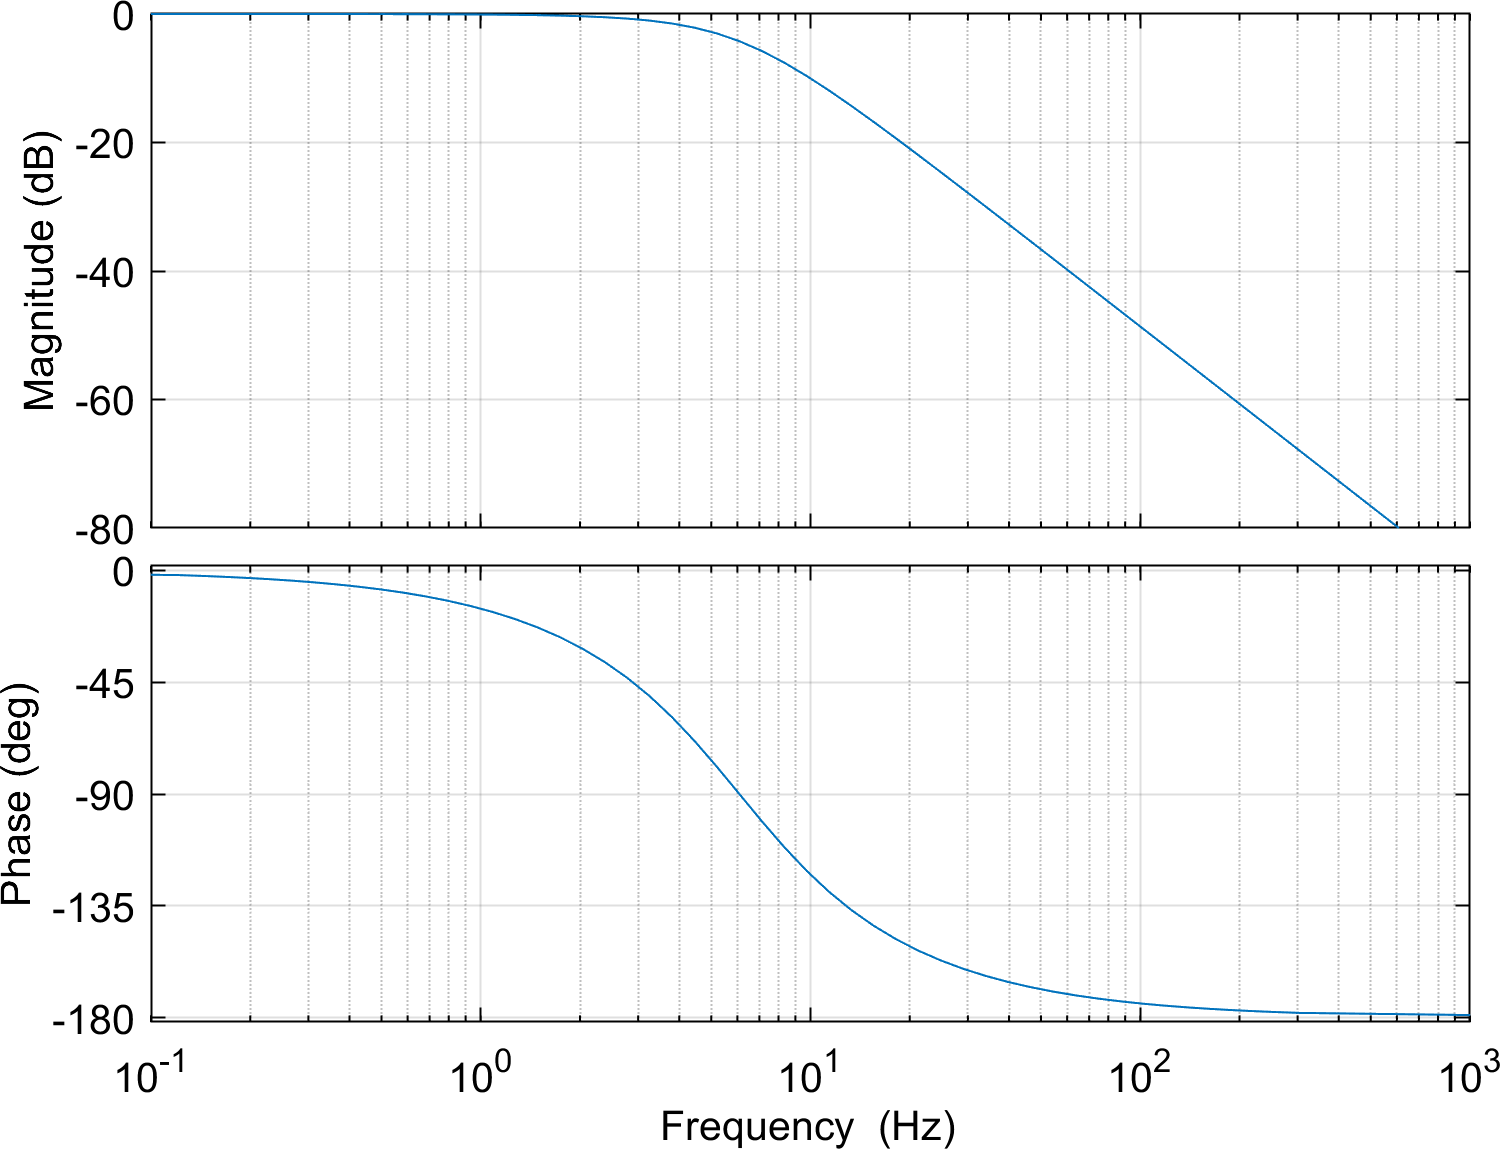
\includegraphics[width=4in]{servoInputDynamics.png}
	\caption{Bode plot of actuator transfer function}
	\label{fig:servoInputDynamics}
\end{figure}
This transfer function was then converted to the following equivalent state-space representation:
\begin{equation}
\begin{aligned}
    \label{eq:servoModel}
    s\{x\} &= \begin{bmatrix} -62.2 & -1461 \\ 1 & 0 \end{bmatrix} \{x\}
        + \begin{bmatrix} 0 \\ 1 \end{bmatrix} u \\
    y &= \begin{bmatrix} 0 & 1461 \end{bmatrix} \{x\}
\end{aligned}
\end{equation}
where $u$ is the input, $y$ is the output, and $\{x\}$ is the internal state of the actuator.

\subsection{Gust Vanes} %%%%%%%%%%%%%%%%%%%%%%%%%%%%%%%%%%

The wind tunnel gust vanes were measured to have ``perfect'' dynamics except for a pure time delay of 0.34 seconds. This pure delay was approximated as a second-order transfer function using a Pad\'e approximant:
\begin{align}
    G(s) &= \frac{s^2 - 176.47s + 10381}{s^2 + 176.47s + 10381}
\end{align}
The Pad\'e approximant matches the pure delay's response well in the frequency range of interest (<20 Hz); the step response and phase shift behavior of a pure delay and the Pad\'e approximant are compared in Fig. \ref{fig:padeApprox}.
\begin{figure}[H]
    \centering
    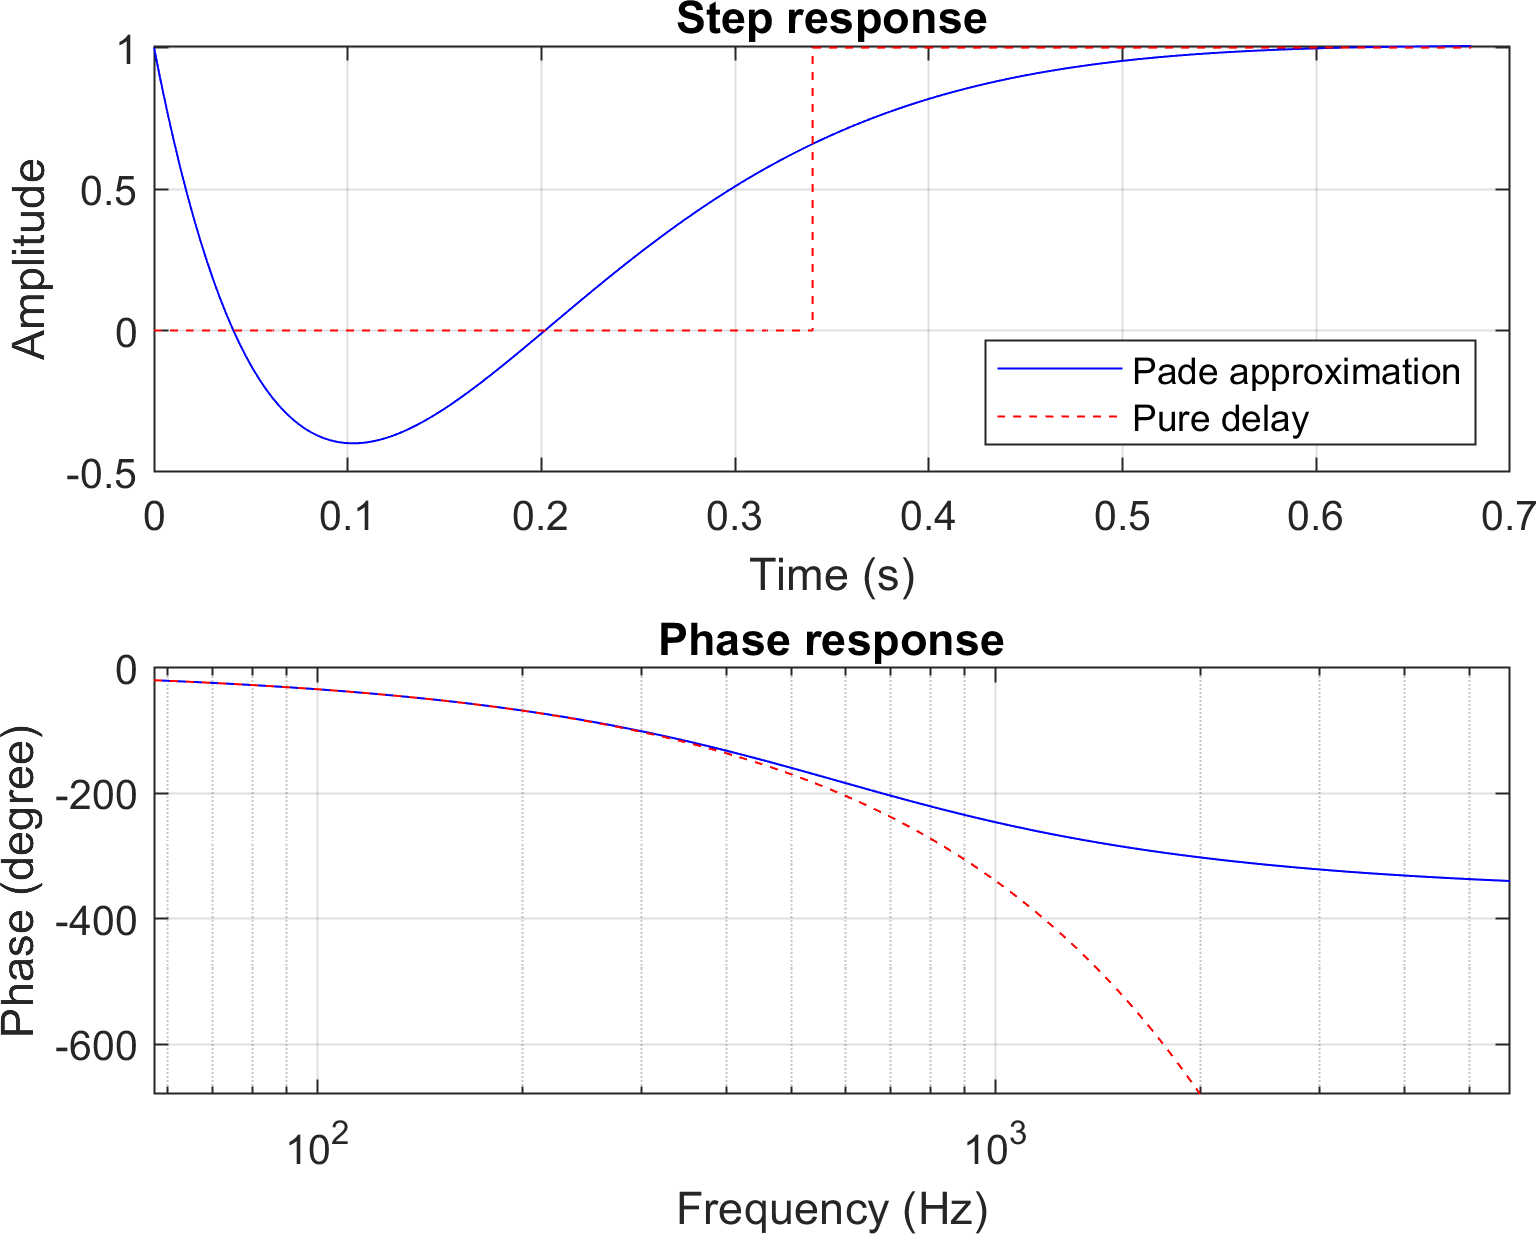
\includegraphics[width=4in]{gustInputDynamics.png}
    \caption{Pad\'e approximant of the pure-delay response of the wind tunnel gust vanes}
    \label{fig:padeApprox}
\end{figure}
This transfer function was then converted to the following equivalent state-space representation:
\begin{equation}
\begin{aligned}
\label{eq:gustModel}
    s\{x\} &= \begin{bmatrix} -176.47 & -10381 \\ 1 & 0 \end{bmatrix} \{x\}
        + \begin{bmatrix} 1 \\ 0 \end{bmatrix} u \\
    y &= \begin{bmatrix} -352.94 & 0 \end{bmatrix} \{x\}
        + \begin{bmatrix} 1 \end{bmatrix} u
\end{aligned}
\end{equation}
where $u$ is the input, $y$ is the output, and $\{x\}$ is the internal state of the actuator.

\subsection{Combined Actuation and Sensing} %%%%%%%%%%%%%%%%%%%%%%%%%%%%%%%%%%

The state-space models for the four actuators (three servo-actuated control surfaces and one pair of wind tunnel gust vanes) are combined to form one combined state-space model for all actuators with input, output, and state
\begin{align}
    \{u_\text{act}\} &= \begin{bmatrix} u_1 \\ u_2 \\ u_3 \\ u_4 \end{bmatrix} &
    \{y_\text{act}\} &= \begin{bmatrix} y_1 \\ y_2 \\ y_3 \\ y_4 \end{bmatrix} &
    \{x_\text{act}\} &= \begin{bmatrix} \{x\}_1 \\ \{x\}_2 \\ \{x\}_3 \\ \{x\}_4 \end{bmatrix}
\end{align}
respectively. The combined actuation state-space model is then
\begin{equation}
\begin{aligned}
    \{x_\text{act}\} &= \begin{bmatrix}
        [A_1] & & & \\ & [A_2] & & \\ & & [A_3] & \\ & & & [A_4]
        \end{bmatrix} \{x_\text{act}\}
        + \begin{bmatrix}
        [B_1] & & & \\ & [B_2] & & \\ & & [B_3] & \\ & & & [B_4]
        \end{bmatrix} \{u_\text{act}\} \\
    \{y_\text{act}\} &= \begin{bmatrix}
        [C_1] & & & \\ & [C_2] & & \\ & & [C_3] & \\ & & & [C_4]
        \end{bmatrix} \{x_\text{act}\}
        + \begin{bmatrix}
        [D_1] & & & \\ & [D_2] & & \\ & & [D_3] & \\ & & & [D_4]
        \end{bmatrix} \{u_\text{act}\}
\end{aligned}
\end{equation}
where the $[A]$, $[B]$, $[C]$, and $[D]$ system matrices for the two types of actuators are defined above in Eq. \ref{eq:servoModel} and \ref{eq:gustModel}. This then forms the actuator block shown in Fig. \ref{fig:actPlantSens}.

A similar process would be appropriate for a set of imperfect sensors. However, the high-rate sensors used in MARGE have approximately no dynamics in the frequency range of interest. Thus, the sensor response was approximated as
\begin{align}
    \{y_\text{sens}\} &= [I] \{u_\text{sens}\}
\end{align}
In other words, the output of the sensor was taken as the output of the plant. This then forms the sensor block shown in Fig. \ref{fig:actPlantSens}.

%%%%%%%%%%%%%%%%%%%%%%%%%%%%%%%%%%%%%%%%%%%%%%%%%%%%%%%%%%%%%%%%%%%%%%%%
\section{Coupled Aeroservoelastic Modeling} %%%%%%%%%%%%%%%%%%%%%%%%%%%%
%%%%%%%%%%%%%%%%%%%%%%%%%%%%%%%%%%%%%%%%%%%%%%%%%%%%%%%%%%%%%%%%%%%%%%%%

The imperfect actuators and sensors can be accounted for in modeling by combining the actuator, plant, and sensor models into an integrated system model that can then be used for control design; see Fig. \ref{fig:actPlantSens} for a block diagram of this system of systems.
\begin{figure}[h]
    \centering
    \includegraphics[width=\textwidth]{ASEblockDiagram.png}
    \caption{Integrated model of actuation, plant, and sensing in a control loop}
    \label{fig:actPlantSens}
\end{figure}
In the system illustration in Fig. \ref{fig:actPlantSens}, the actuators take in the control command and output control forces; the plant takes in control forces and outputs motions; the sensors take in motions and output measured motions; and a control law can then use this measured motion to create a control command for MARGE.

First, the actuator dynamics can be coupled to the plant dynamics. In state-space form, this is
\begin{align}
	\label{eq:coupledState}
	s \begin{Bmatrix} \{x_\text{act}\} \\ \{x_p\} \end{Bmatrix} &= \begin{bmatrix}
		[A_\text{act}] & [0] \\
		[B_p] [C_\text{act}] & [A_p]
	\end{bmatrix} \begin{Bmatrix} \{x_\text{act}\} \\ \{x_p\} \end{Bmatrix}
	+ \begin{bmatrix} [B_\text{act}] \\ [B_p][D_\text{act}] \end{bmatrix} \{u_\text{act}\}
\end{align}
where the entries in the block matrices containing $[B_p]$ are used to convert $\{x_\text{act}\}$ and $\{u_\text{act}\}$ into the plant's input, $\{u_p\}=\{y_\text{act}\}$.

The actuator can similarly be coupled to the plant in the output equations:
\begin{align}
	\label{eq:coupledOutput}
	\{y_p\} &= \begin{bmatrix}
		[D_p][C_\text{act}] & [C_p]
	\end{bmatrix} \begin{Bmatrix} \{x_\text{act}\} \\ \{x_p\} \end{Bmatrix}
	+ [D_p] [D_\text{act}] \{u_\text{act}\}
\end{align}
where similarly, the terms involving $[D_p]$ are used to convert $\{x_\text{act}\}$ and $\{u_\text{act}\}$ into the plant's input, $\{u_p\}=\{y_\text{act}\}$.

The block matrices in Eq. \ref{eq:coupledState} and \ref{eq:coupledOutput} form the coupled actuator-plant system in Fig. \ref{fig:actPlantSens}. Since the sensors are modeled as perfect, this is also equivalent to the coupled actuator-plant-sensor system. Thus, Eq. \ref{eq:coupledState} and \ref{eq:coupledOutput} define the state-full, coupled space model for MARGE in the form required as defined in Eq. \ref{eq:modelingGoal}.